\chapter{Preparation}\label{ch:prep}

This chapter gives the background needed to understand the design of Veritas: the type-system machinery used to express safety properties, the related verification systems that informed the design, and the engineering decisions that fix the project's trust boundary. The aim is to establish only the theory and design context needed for the implementation that follows.

\section{Background}\label{sec:background}

\subsection{Type systems and safety}

The fundamental theorem that connects type systems to safety is \emph{type soundness}: a well-typed program cannot `go wrong' at runtime~\cite{Milner1978Theory}. Wright and Felleisen formalised this via the \emph{progress} and \emph{preservation} lemmas~\cite{Wright1994Syntactic}:

\begin{center}
\small
\begin{tabularx}{0.94\textwidth}{>{\raggedright\arraybackslash}p{0.22\textwidth} >{\raggedright\arraybackslash}X}
\toprule
\textbf{Progress} & If $\emptyset \vdash e : \tau$, then either $e$ is already a value, or there exists some expression $e'$ such that $e \to e'$. \\
\textbf{Preservation} & If $\emptyset \vdash e : \tau$ and $e \to e'$, then $\emptyset \vdash e' : \tau$. \\
\bottomrule
\end{tabularx}
\end{center}

\noindent Starting from a well-typed program, repeated evaluation can neither get stuck in an ill-defined intermediate state (progress) nor escape the guarantees expressed by its type (preservation). In practice, this is the formal basis for claims such as ``a well-typed array access cannot go out of bounds''.

The relevant distinction for Veritas is whether a type system can express facts about values, not only broad categories of values. Ordinary type systems classify values as integers, booleans, pointers, or polymorphic structures. Refinement and dependent type systems can also state that a particular integer is positive, that an index is in bounds, or that an array has a fixed length.

\subsection{Dependent types and refinement types}\label{sec:dependent-types}

\term{Dependent types} allow types to depend on terms. The canonical example is a vector type indexed by its length, $\mathrm{Vec}(A, n)$. A lookup function can require in its type that the index is valid:
\[
  \mathrm{lookup} :
  \mathrm{Vec}(A,n) \to
  \{i\!:\!\mathtt{int} \mid 0 \le i < n\} \to A
\]
Full dependent type systems, such as those in Coq and Agda~\cite{Bove2009Agda}, can express arbitrary propositions as types, but this generality comes at a cost: type checking is expensive and may require the programmer to construct explicit proof terms.

\term{Refinement types}~\cite{Rondon2008Liquid} are a practical restriction of full dependent types. A base type is decorated with a logical predicate drawn from a decidable logic, for example $\{v\!:\!\mathtt{int} \mid v > 0\}$. Subtyping between refinement types reduces to logical implication:
\[
  \{v\!:\!\mathtt{int} \mid P(v)\}
  <:
  \{v\!:\!\mathtt{int} \mid Q(v)\}
  \quad\text{when}\quad
  P(v) \Rightarrow Q(v)
\]
This turns refinement subtyping into an SMT obligation.

A particularly useful special case is the \term{singleton type}, written $\mathtt{int}(n)$, which is inhabited by exactly the integer $n$. Singleton types arise naturally from Xi and Pfenning's work on Dependent ML~\cite{Xi1999DML}, where integer index expressions are used to track array sizes and loop bounds. Singleton types can propagate exact values through arithmetic:
\[
  \begin{array}{rcl}
    x &:& \mathtt{int}(3) \\
    y &:& \mathtt{int}(5) \\
    x + y &:& \mathtt{int}(8)
  \end{array}
\]
This enables compile-time verification of array bounds when indices are statically known.

\subsection{Bidirectional type checking}

Bidirectional type checking~\cite{Pierce2000Local} structures type checking into two mutually recursive judgements:

\begin{center}
\small
\begin{tabularx}{0.94\textwidth}{>{\raggedright\arraybackslash}p{0.25\textwidth} >{\raggedright\arraybackslash}X}
\toprule
\textbf{Type checking} & Verifies that expression $e$ has expected type $\tau$: $\Gamma \vdash e \leftarrow \tau$. \\
\textbf{Type synthesis} & Infers a type $\tau$ for expression $e$: $\Gamma \vdash e \Rightarrow \tau$. \\
\bottomrule
\end{tabularx}
\end{center}
\noindent The two modes are connected by a subsumption rule:
$$
  \frac{\Gamma \vdash e \Rightarrow \sigma \quad \sigma <: \tau}{\Gamma \vdash e \leftarrow \tau}
$$
For refinement types, synthesis can produce precise local facts: integer literals synthesise singleton types, and arithmetic synthesises refinements relating the result to its operands. Checking then verifies subtyping against the expected type. In Veritas, programmers annotate function boundaries and mutable declarations; intermediate refinements are inferred.

The same structure also threads the typing context through the judgements, reflecting mutable assignments and newly learned refinement propositions.

\subsection{SMT-based verification}
\label{sec:smt-based-ver}

Satisfiability Modulo Theories (SMT) solvers check satisfiability of formulae over richer logics than propositional SAT. Veritas uses Z3~\cite{DeMoura2008Z3} for linear integer arithmetic, arrays, uninterpreted functions, and bounded quantifiers over array specifications.

The technique for using an SMT solver as a refinement type checker is \term{proof by refutation}~\cite{Rondon2008Liquid}. To check whether $\phi \vdash P$ holds, Veritas checks whether $\phi \wedge \lnot P$ is unsatisfiable:

\[
  \phi \vdash P
  \quad\text{iff}\quad
  \phi \wedge \lnot P \text{ is unsatisfiable}
\]

This approach means that proof obligations are discharged automatically: the programmer supplies type annotations, function contracts, and loop invariants, but never constructs proof terms. In Veritas, the SMT solver is invoked for refinement subtyping, array bounds verification, and function contract verification at call sites and return points.

\subsection{Type-preserving compilation and proof-carrying code}\label{sec:type-pres-background}

Conventional compilers erase types after type checking, discarding the safety guarantees established by the type system. The generated machine code is subsequently trusted on the basis that the compiler is correct, an assumption that is difficult to verify for large, complex compilers. Type-preserving compilation~\cite{Morrisett1999SystemF} retains type information through every intermediate representation in the pipeline. This enables the property that the compiled output can be independently verified without trusting the compiler. If a bug in the compiler produces type-incorrect code, the type annotations on the output will be inconsistent, and the verifier will reject it.

The idea of shipping machine code together with a checkable proof of its safety was formalised by Necula as proof-carrying code (PCC)~\cite{Necula1997PCC}. In PCC, the code producer generates executable code and a safety proof; the code consumer checks the proof against a safety policy before execution. Type-preserving compilation can be seen as a particular instance of PCC where the `proof' takes the form of type annotations.

\subsection{Dependently Typed Assembly}\label{sec:dtal-background}

Xi and Harper introduced DTAL as a target for type-preserving compilation from DML and Xanadu~\cite{Xi1999DML,Xi2000Xanadu}. DTAL augments assembly with two key forms of type annotation:
\begin{itemize}
  \item \textbf{Label signatures}: each basic block entry point is annotated with existentially quantified index variables and the types expected for each register on entry, enabling modular, block-by-block verification.
  \item \textbf{Register types}: types may depend on index variables, so that a register's type tracks its exact value (e.g., $\mathtt{int}(i)$) or the size of an array it points to (e.g., $\mathtt{int\;array}(n)$).
\end{itemize}

\noindent A DTAL loop header binds index variables and declares register types in terms of them:

\begin{verbatim}
  loop:  {m:nat, n:nat | m <= n, i:nat}
         [r1: int array(m), r2: int array(n), r3: int(m), r4: int(i)]
         sub   r5, r4, r3       // r5 <- i - m
         bgte  r5, finish       // if i >= m, exit
         load  r5, r1(r4)       // safe: i < m
         store r2(r4), r5       // safe: i < n (since m <= n)
         add   r4, r4, 1
         jmp   loop
\end{verbatim}

\noindent The branch \texttt{bgte r5, finish} refines the type state: on the fall-through path, the type system knows $i < m$, which makes the subsequent \texttt{load} and \texttt{store} provably safe without any runtime bounds check. Xi and Harper proved that well-typed DTAL programs cannot violate the constraints of the type system.

Veritas implements its own DTAL variant based on Xi and Harper's design, extended to support the Veritas refinement type system and x86-64. The compiler translates source through a typed intermediate representation (TIR) to DTAL, preserving refinement types at each stage, and finally emits x86-64 machine code as an ELF executable. Hereafter, `DTAL' refers to this Veritas-specific variant unless otherwise noted; the original is referred to as `Xi and Harper's DTAL'.

\section{Related work and design influences}
\label{sec:related-work}

Veritas combines automated refinement checking, systems-language design, and proof-carrying code. The systems below matter because each fixes a different point in the design space: automation, expressiveness, systems orientation, or low-level trust.

\subsection{Refinement types and automated verification}
Liquid Haskell~\cite{Vazou2014Refinement} and Liquid Types~\cite{Rondon2008Liquid} provide the main precedent for SMT-backed refinement checking. Dafny~\cite{Leino2010Dafny} similarly uses SMT solving for imperative contracts and loop invariants. Veritas borrows this style of automatic proof discharge, but preserves the resulting constraints down to assembly rather than erasing them after source-level verification.

\subsection{Foundational and dependent verification}
F*~\cite{Swamy2016Dependent} and RefinedC~\cite{Sammler2021RefinedC} offer stronger theoretical foundations through dependent types or separation logic. RefinedC, for example, produces machine-checked Coq proofs for existing C code. Veritas deliberately accepts a weaker foundation, SMT-backed checking rather than foundational proof, to keep proof obligations automatic once specifications are supplied.

\subsection{Verifiable systems languages}
ATS (Applied Type System)~\cite{Xi2003Applied} is the closest predecessor in spirit: it targets systems programming with dependent types and zero runtime overhead. The key difference is architectural. ATS proves properties at compile time and then emits C, leaving the ATS and C compilers in the TCB. Veritas instead preserves types into DTAL so that the low-level target can be checked independently.

The recurring difference is not whether verification is possible, but where the evidence is checked and what remains trusted after compilation. Figure~\ref{fig:verification-landscape} summarises the trade-off between expressiveness and automation across the systems discussed above.

\begin{figure}[H]
  \centering
  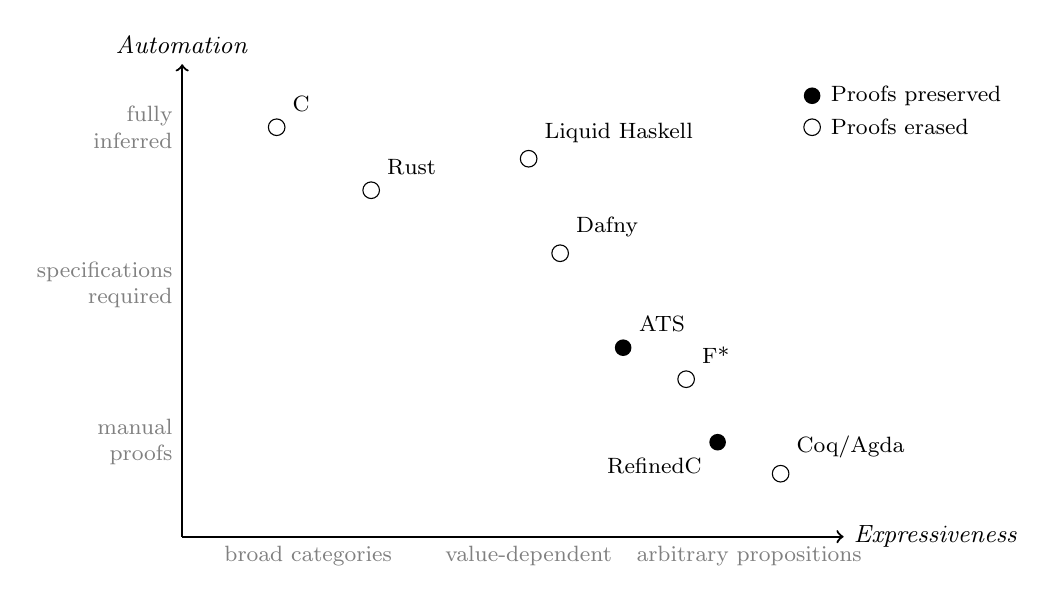
\begin{tikzpicture}[
      every node/.style={font=\small},
      filled/.style={circle, fill=black, inner sep=0pt, minimum size=6pt},
      hollow/.style={circle, draw=black, fill=white, inner sep=0pt, minimum size=6pt},scale=0.8
    ]
    \draw[->, thick] (0,0) -- (10.5,0) node[right] {\textit{Expressiveness}};
    \draw[->, thick] (0,0) -- (0,7.5) node[above] {\textit{Automation}};

    \node[below left, font=\footnotesize] at (0,0) {};
    \node[below, font=\footnotesize, text=gray] at (2,0) {broad categories};
    \node[below, font=\footnotesize, text=gray] at (5.5,0) {value-dependent};
    \node[below, font=\footnotesize, text=gray] at (9,0) {arbitrary propositions};
    \node[left, font=\footnotesize, text=gray, align=right] at (0,1.5) {manual\\proofs};
    \node[left, font=\footnotesize, text=gray, align=right] at (0,4) {specifications\\required};
    \node[left, font=\footnotesize, text=gray, align=right] at (0,6.5) {fully\\inferred};

    \node[hollow, label={[font=\footnotesize]above right:C}] at (1.5,6.5) {};

    \node[hollow, label={[font=\footnotesize]above right:Rust}] at (3,5.5) {};

    \node[hollow, label={[font=\footnotesize]above right:Liquid Haskell}] at (5.5,6) {};

    \node[hollow, label={[font=\footnotesize]above right:Dafny}] at (6,4.5) {};


    \node[filled, label={[font=\footnotesize]above right:ATS}] at (7,3) {};

    \node[hollow, label={[font=\footnotesize]above right:F*}] at (8,2.5) {};

    \node[filled, label={[font=\footnotesize]below left:RefinedC}] at (8.5,1.5) {};

    \node[hollow, label={[font=\footnotesize]above right:Coq/Agda}] at (9.5,1) {};

    \node[filled, label={[font=\footnotesize]right:Proofs preserved}] at (10,7) {};
    \node[hollow, label={[font=\footnotesize]right:Proofs erased}] at (10,6.5) {};

  \end{tikzpicture}
  \caption{Verification systems positioned by expressiveness of their type/specification language and degree of automation.}
  \label{fig:verification-landscape}
\end{figure}

\section{Requirements and success criteria}\label{sec:requirements-anal}

The requirements define what counts as success for Veritas: the language must express useful safety properties, the compiler must preserve evidence for those properties, and the generated low-level code must be checkable independently of the compiler. They were categorised using the MoSCoW method to keep the project focused on type-preserving compilation and independent low-level verification.

\begin{table}[H]
  \centering
  \small
  \begin{tabularx}{0.94\textwidth}{>{\raggedright\arraybackslash}p{0.16\textwidth} >{\raggedright\arraybackslash}X}
    \hline
    \textbf{Priority} & \textbf{Requirements} \\
    \hline
    Must-have & Variables, control flow, functions, arrays, refinement and singleton types; SMT-backed checking; type-preserving compilation to DTAL; a standalone verifier for generated assembly. \\
    Should-have & Native x86-64 ELF generation; function contracts with postconditions and quantified specifications; tests for accepted safe programs and rejected unsafe programs. \\
    Could-have & Backend optimisations; structs; generics; a full ownership model; a DTAL interpreter. \\
    Won't-have & A machine-checked compiler correctness proof; concurrency verification; information-flow or cryptographic verification. \\
    \hline
  \end{tabularx}
  \caption{MoSCoW requirements.}
  \label{tab:moscow-requirements}
\end{table}

\begin{center}
\small
\begin{tabularx}{0.94\textwidth}{>{\raggedright\arraybackslash}p{0.22\textwidth} >{\raggedright\arraybackslash}X}
\toprule
\textbf{Success criterion} & \textbf{Meaning} \\
\midrule
Expressiveness & Source-level safety properties can be expressed. \\
Preservation & Safety evidence is preserved through compilation to DTAL. \\
Independent rejection & Unsafe generated low-level code is rejected independently of the compiler. \\
Executable output & Accepted programs can be emitted and run as x86-64 ELF binaries. \\
\bottomrule
\end{tabularx}
\end{center}

\section{Design decisions}\label{sec:design-decisions}

The central design task was to realise this trust architecture without making the source language unusable or the trusted backend too large.

\subsection{Trust model and compiler architecture}

A central architectural decision is that the compiler is \textit{untrusted}. Rather than proving the compiler correct, Veritas relies on a standalone verifier that re-checks the compiler's low-level output. Compiler bugs should therefore cause rejection, not unsafely accepted code. Figure~\ref{fig:trust-pipeline} shows the resulting boundary: type information flows through the compiler, but trust begins only at the verifier and direct encoder.

The implementation moved the verification boundary progressively lower: first checking virtual DTAL, then physical DTAL after register allocation, and finally keeping the runtime small enough to audit by inspection, with a bare-metal target removing the OS from the TCB.

\begin{figure}[H]
  \centering
  \begin{tikzpicture}[
      scale=0.85,
      transform shape,
      node distance=0.9cm and 1.1cm,
      box/.style={draw, rounded corners, minimum height=1.0cm, minimum width=4.0cm, align=center, font=\small},
      typed/.style={box, fill=blue!10},
      untyped/.style={box, fill=gray!10},
      trusted/.style={box, fill=green!12},
      arrow/.style={-Latex, thick}
    ]
    \node[untyped] (src) {Source\\\texttt{.veri}};
    \node[typed, right=of src] (tast) {Typed AST};
    \node[typed, right=of tast] (tir) {Typed SSA\\(TIR)};
    \node[typed, right=of tir] (dtal) {DTAL};

    \node[typed, below=1.6cm of dtal] (phys) {Physical DTAL};
    \node[trusted, left=of phys] (verifier) {Independent Verifier};
    \node[trusted, left=of verifier] (encoder) {Direct Encoder};
    \node[untyped, left=of encoder] (elf) {ELF / Machine Code};

    \draw[arrow] (src) -- (tast);
    \draw[arrow] (tast) -- (tir);
    \draw[arrow] (tir) -- (dtal);
    \draw[arrow] (dtal) -- node[right=0.35cm, font=\scriptsize, align=left, fill=white, inner sep=1pt] {physalloc\\(untrusted)} (phys);
    \draw[arrow] (phys) -- (verifier);
    \draw[arrow] (verifier) -- (encoder);
    \draw[arrow] (encoder) -- (elf);

    \draw[dashed, rounded corners]
    ([xshift=-0.35cm,yshift=0.35cm]tast.north west) --
    ([xshift=0.35cm,yshift=0.35cm]dtal.north east) --
    ([xshift=0.35cm,yshift=-0.35cm]dtal.south east) --
    ([xshift=0.35cm,yshift=-0.35cm]phys.south east) --
    ([xshift=-0.35cm,yshift=-0.35cm]phys.south west) --
    ([xshift=-0.35cm,yshift=-0.35cm]dtal.south west) --
    ([xshift=-0.35cm,yshift=-0.35cm]tast.south west) --
    ([xshift=-0.35cm,yshift=0.35cm]tast.north west);
    \node[font=\small, above] at ([yshift=0.35cm]tir.north) {untrusted compiler};
    \node[draw, dashed, rounded corners, fit=(verifier)(encoder), inner sep=0.25cm,
      label={[font=\small]below:trusted core}] {};
  \end{tikzpicture}
  \caption{Veritas compilation pipeline and trust boundary. The final design verifies physical DTAL, so register allocation and instruction selection remain outside the trusted core.}
  \label{fig:trust-pipeline}
\end{figure}

\subsection{Language and target choices}\label{sec:prep-language-target}

\prepblock{Source language}{Veritas is a small imperative language with C-like syntax, inspired by Xi and Harper's Xanadu. It supports integers, booleans, fixed-size arrays, mutable and immutable variables, loops, and functions. The type system adds singleton types, refinement types, contracts, bounded quantifiers, and loop invariants.}

\prepblock{Bounded quantification}{Scalar refinements can prove facts about individual values, but algorithms such as binary search need array-wide properties such as sortedness. A precondition such as $\mathbf{forall}\ i\ \mathbf{in}\ 0..n\ \{\ \mathit{arr}[i] \le \mathit{arr}[i + 1]\ \}$ expresses such properties while keeping verification close to SMT-friendly fragments.}

\prepblock{DTAL target}{The target language is a variant of Xi and Harper's DTAL~\cite{Xi2001DTAL}, extended for Veritas refinements and x86-64. The core instruction set is deliberately RISC-like: simple instructions are easier to type, verify, and map from the SSA-style intermediate representation. DTAL then adds register type annotations, embedded constraint assertions, and declared type states at basic block entries.}

\prepblock{Physical register model}{I also defined DTAL with its own \term{physical register model} (registers \texttt{r0}--\texttt{r12}, \texttt{sp}, \texttt{fp}, \texttt{lr}) that maps directly to x86-64 registers. This allows verification to occur \term{after} register allocation: the register allocator is untrusted, and its output is verified before the final encoding to x86-64.}

\prepblock{Direct encoding}{Rather than emitting assembly text and invoking NASM or GAS, Veritas encodes x86-64 instructions directly as bytes. This keeps an external assembler out of the TCB and enables direct execution on the development machine. The trusted path below physical DTAL is intentionally small: a one-to-one instruction mapping, a byte encoder, and an ELF generator.}

\subsection{Design challenges}\label{sec:design-challenges}

Four design challenges shaped the implementation:

\challengeblock{Mutable variables and refinement types}{Refinement type systems such as Liquid Haskell operate over immutable bindings, where a variable's type is fixed at its definition. Supporting mutation introduces a soundness hazard: after \texttt{x = e}, any refinement mentioning \texttt{x} may be invalidated.}{The solution adopted, \term{master types}, required designing the mutable context $\Delta$ to track both a current type and a fixed master type, with a subtyping check on every assignment.}{This keeps refinements sound in the presence of assignment.}

\challengeblock{Verification after register allocation}{The initial system verified DTAL with virtual registers and then trusted the x86-64 lowering ($\sim$1,100 lines of register allocation, instruction selection, and encoding).}{Redesigning the pipeline to verify \term{after} register allocation required a physical DTAL register model, an untrusted allocation pass, a direct encoder, and verifier support for physical instructions.}{This reduced the trusted backend code to $\sim$300 lines.}

\challengeblock{Type preservation across SSA join points}{At phi nodes in the SSA intermediate representation, two singleton types from different branches (e.g., $\mathtt{int}(3)$ and $\mathtt{int}(7)$) must be joined. Widening to the base type $\mathtt{int}$ loses refinement information, making downstream bounds proofs impossible.}{The solution was to attach \term{existential constraints} to phi nodes, encoding that the value satisfies a constraint without fixing it to a concrete value.}{This mechanism was not part of Xi and Harper's original DTAL design and required extending both the TIR and the verifier.}

\challengeblock{SMT encoding of array properties}{Verifying array-manipulating programs requires reasoning about array contents, which involves quantified formulae. These fall outside the decidable quantifier-free fragment of linear integer arithmetic.}{The design restricted quantifiers to \term{bounded} forms ($\mathbf{forall}\ x\ \mathbf{in}\ a..b$), which Z3's E-matching heuristics handle reliably in practice.}{This excludes unbounded quantification, but maintains the automatability of verification.}

\section{Project management and starting point}
\label{sec:software-eng-methodology}

\prepblock{Development process}{The implementation followed an incremental pipeline-first strategy. I first built an end-to-end compiler for integer arithmetic, then extended the same path with arrays, mutation, refinements, contracts, and quantifiers. Each feature was accompanied by positive tests that should compile and negative tests that should be rejected with a specific error.}

\prepblock{Engineering process and tools}{Version control was managed using Git, with short-lived feature branches merged into the main branch. A GitHub Actions CI pipeline ran on each push, enforcing \texttt{cargo fmt}, \texttt{cargo clippy}, example validation, and the test suite on Ubuntu Linux and macOS. The project was implemented in Rust; the frontend type checker and DTAL verifier use Z3 via the \texttt{z3} Rust crate, and \texttt{im} provides persistent data structures for typing contexts.}

\prepblock{Professional practice}{The project used open-source dependencies whose licences were checked before inclusion and are listed where they affect the implementation boundary. The evaluation uses generated programs, authored examples, and public benchmark kernels rather than personal data or human-subject data, so data-protection and human-subject concerns are minimal. The main consequence of the work is research-facing: it explores how safety evidence can be preserved into low-level code, which could reduce trust in compiler infrastructure if developed further.}

\prepblock{Starting point}{I began with introductory knowledge of dependent type theory and verification languages, and was introduced to refinement types through Xi and Harper's DTAL. No external compiler or verifier code was used. The main new areas were Rust, SMT-backed type checking, Z3 theories, x86-64 encoding, bidirectional type checking, and the Xi et al. papers on DML, Xanadu, and DTAL.}
